
\begin{His}

Le  vocable même de «  fonction  »  n’est apparu que tardivement (fin   XVIIIesiècle). Le concept, par contre, s’est dégagé petit à petit dans quelques ouvrages tels : « La latitude des formes » d’Oresme (XIVe  siècle), l’étude de \textsc{Galilée} sur la  dépendance de la  vitesse  par  rapport au temps (vers 1640), les expressions algébriques liées    aux courbes chez \textsc{Descartes} (à la même époque).

\vspace{0.4cm}

Dans l’Antiquité, il peut même être repéré dans la  confection des tables des cordes  liées  aux arcs de cercle (les ancêtres de nos sinus). Les  nombreuses tables  de  calcul  publiées durant le XVIe siècle constituent également une approche significative. 

\vspace{0.4cm}
Mais  lorsque,  s’exprimant en latin,  le « géomètre» disait    que,    dans    une    expression,  une  quantité contenant  deux  grandeurs,  on  pouvait  calculer l’une à partir de l’autre, il ne lui était pas nécessaire de faire appel à un mot particulier, un   cas de déclinaison grammaticale pouvait suffire ; au plus usait-il d’une préposition (a, ab, ex). 

\textsc{Newton}, qui rédigeait en latin, semble avoir été le premier, vers 1670, à formuler un terme propre en usant du mot « genita » pour désigner une quantité obtenue, engendrée, à partir d’autres quantités et ce, au moyen des quatre opérations. 

\vspace{0.4cm}

\begin{wrapfigure}[15]{r}{3.6cm}
\vspace{-7mm}
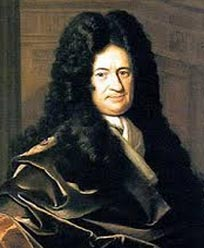
\includegraphics[scale=0.5]{image_chapitres/liebniz.jpg}
\unnumberedcaption{G. W. \textsc{Leibniz}} 
\end{wrapfigure}
\textbf{\textsc{Gottfried Wilhelm Leibniz}},  dans  deux  textes  en  latin  des  « \textit{Acta  cruditorum}  »  de  1673  et  1692,  use  du vocable  «  \textit{functio, functiones} », mot  forgé  à  partir  du  participe  passé  du  verbe \textit{fungor}   (accomplir,   remplir   une  
charge).  Puis  il  francise  le  mot.  Dans  le  « \textit{Journal des sçavans} » de 1694, il écrit (en   français)   :   «   entre   deux  fonctions   quelconques de la ligne AC... ». Et plus  loin  suit  une  définition  en  lien  avec  la  question    étudiée    alors    :  " J’appelle fonction  toutes  les  portions  de  lignes qu’on  fait  en  menant... ".  Ailleurs  il  désigne,  toujours  en  français,  l’abscisse,  l’ordonnée,  la  corde  comme  fonctions  d’une courbe.

\vspace{0.4cm}
Le terme fut alors repris par d’autres. En juillet 1698,  Leibniz écrit à  Jean Bernoulli :   «   J’ai   plaisir   à   vous   voir   
employer  le  terme  fonction  dans  mon  sens  ».  Et  Bernoulli  de  lui  répondre  de  Groningen  au  mois  d'aout  «  Pour  noter  
une   fonction   d’une   certaine   quantité indéterminée $x$, j’aime  utiliser  la majuscule  correspondante  $X$  ou  la lettre  grecque $\zeta$. On peut voir immédiatement de quelle indéterminée dépend la fonction. » 

\vspace{0.4cm}

Le  concept  perd  alors,  petit  à  petit,  son  caractère géométrique immédiat. Dans  les  « \textit{ Mémoires  de  l’Académie  des 
Sciences} », en 1718, Bernoulli écrit : 

« DÉFINITION  :    On  appelle  ici FONCTION  d’une  grandeur  variable, une   quantité   composée   de   quelque   manière  que  ce  soit  de  cette  grandeur  variable et de constantes. » 

\vspace{0.4cm}

Euler prend la suite et, dans une note de l’Académie de Saint Petersbourg (1734), il  introduit  la  notation  $f\left( \frac{x}{a}+c \right)$ pour : « un fonction arbitraire de $\frac{x}{a}+c$».
 
\PESP{http://www.apmep.fr/IMG/pdf/Fonctions.pdf}
 
\end{His}
